\documentclass{anstrans}
%%%%%%%%%%%%%%%%%%%%%%%%%%%%%%%%%%%
\title{Evidence of the necessity of isotopic precise calculation in fuel cycle
calculation}
\author{Baptiste Mouginot$^{*}$, Paul P.H. Wilson$^{*}$, Robert W. Carlsen$^{*}$, Meghan B. McGarry$^{*}$,
Arrielle C. Opotowsky$^{*}$ }

\institute{
$^{*}$University of Wisconsin-Madison, WI
\and
%$^{\dagger}$State Capitol Building, Springfield, IL
}

\email{mouginot@wisc.edu \and paul.wilson@wisc.edu}

% Optional disclaimer: remove this command to hide
%\disclaimer{Notice: this manuscript is a work of fiction. Any resemblance to
%actual articles, living or dead, is purely coincidental.}

%%%% packages and definitions (optional)
\usepackage{graphicx} % allows inclusion of graphics
\usepackage{booktabs} % nice rules (thick lines) for tables
\usepackage{microtype} % improves typography for PDF

\newcommand{\SN}{S$_N$}
\renewcommand{\vec}[1]{\bm{#1}} %vector is bold italic
\newcommand{\vd}{\bm{\cdot}} % slightly bold vector dot
\newcommand{\grad}{\vec{\nabla}} % gradient
\newcommand{\ud}{\mathop{}\!\mathrm{d}} % upright derivative symbol

\begin{document}
%%%%%%%%%%%%%%%%%%%%%%%%%%%%%%%%%%%%%%%%%%%%%%%%%%%%%%%%%%%%%%%%%%%%%%%%%%%%%%%%
\section{Introduction} 

This work is part of the evaluation study of the transition analysis
\cite{Bo} identify as the ``Evaluation Group 29'' or ``EG29'', in the
recently-published Evaluation and Screening (E\&S) \cite{ES}.  The EG29 fuel
cycle corresponds to a double strata fleet. The first stratum is composed by
sodium-cooled fast reactor (SFRs) multi-recycling the plutonium. The surplus
amounts of plutonium is send to the second stratum composed of pressurized water
reactor with full mixed oxide (U/Pu)O$_{2}$ cores (MOX-PWRs).  The PWR stratum
is also multi recycling its plutonium. The target energy generation ratio for
the final EG29 system is 70:30 (SFR:PWR), with a 1\% annual growth in nuclear
energy demand.

The purpose of this study is to enlighten the importance of the isotopic
composition for the plutonium, on PWR MOX fuel fabrication and the effect of its
evolution. Two main effect can modify the isotopic composition of the plutonium
used to build the PWR-MOX fuel: decay and depletion.

All the calculation of this study have been performed using the Cyclus fuel cycle
tool\cite{CYCLUS}. The model used are coming from the Cycamore package, developed by the
Cyclus team (containing the Pu-Equivalent fuel fabrication modeling as well as
the simple fix mixing ratio fuel fabrication). The neural network model have
been included into the Cyclus environment using the cyCLASS tool, allowing to
using all the fuel fabrication model and the depletion model from the CLASS tool
\cite{CLASS} in Cyclus.

\section{Study description}
This works compares the plutonium amount require to build the fresh MOX fuel
using 3 different fabrication modeling: ``fixed mixing ratio'', ``plutonium
equivalent theory'', ``Neural network \cite{Leniau2015125}'', considering or not
decay, and using recipe reactor or recalculation the depletion for each loaded
fuel.

The first part of the study in focused on the effect of the decay on the
isotopic composition of the reprocessed plutonium and its implication of fuel
fabrication depending on the fabrication modeling.
The second part of the study, compares 2 recipes compositions versus recalculated
depletion using the neural network fuel fabrication modeling. 

\subsection{Cycle}
The cycle used for the following study is a very simple cycle implying a single
PWR reactor using MOX fuel. After irradiation the uranium and the plutonium are
separated and re-processed to fuel the next batch of MOX fuel for the PWR.

\begin{figure}[ht] % replace 't' with 'b' to force it to be on the bottom
  \centering
  \includegraphics[width=0.48\textwidth]{flow}
  \caption{Schematic representation of the fuel cycle. Quantities on the row
  represents the cumulative amount in kg of material exchanged between two
facilities in the calculation using ``pu-equivalent'' for fuel fabrication
modeling with decay activated.}
  \label{fig:flow}
\end{figure}

A stream of ``good'' quality plutonium coming from an hypothetical irradiated
SFR blanket is represented by a storage. The impact of the decay on this storage
is limited, as the content in $^{241}$Pu is almost negligible.  In order to
build the first batch of fuel, an initial storage has also been set.  In order
to limit the effect of decay of this storage the initial inventory have been
tuned to be as small as possible (preventing any unnecessary plutonium pilling
up).

\subsection{Fabrication model}
Three different way to model the fuel fabrication have been used: ``fix mixing
ratio'', ``Pu-equivalent`` and ''Neural Network``.
The fix mixing ratio used pre-set ratio for the different stream mixing. The
''Pu-equivalent`` model try to fix the best mixing ratio allowing to reproduce
the initial reactivity of the requested MOX fuel. As the requested fuel
composition correspond to the fuel composition built with the ''fix mixing
ratio`` model, the results of those 2 models are expected to be close.
The last model use a different approach to mix the different stream: the
$<k_{infty}>$, the mean infinity neutronic multiplication factor, have to reach
a threshold at the end of the irradiation ($50~$GWd/t in this study). The
$<k_{infty}>$ used in this study is 1.034 \cite{???}. The Neural Network in this
model have been pre-trained on several different depletion calculation,
allowing it to predict the correct plutonium enrichment required.

Because of all those model have not necessary been tuned on exactly the same
PWR configuration and parameter, only the behavior differences between the
different calculations should be analysed..


The second part of the study compares the amount of plutonium require to build
the PWR-MOX fuel (using the neural network modeling for fuel fabrication) for
the recipe based output composition versus the depletion calculation one.
To redo the depletion calculation for each fuel loaded in the PWR reactor, an
other neural network is used to predict the macroscopic cross section of the
fuel \cite{Leniau2015125} (only fission, capture and n,2n reactions are considered). The
depletion calculation is done renormalizing the neutron flux to maintain a
constant power in the reactor.


%%%%%%%%%%%%%%%%%%%%%%%%%%%%%%%%%%%%%%%%%%%%%%%%%%%%%%%%%%%%%%%%%%%%%%%%%%%%%%%%
\section{Decay}


As observed on Fig. \ref{fig:nod}, despite the different model were not tuned to
describe the exact same PWR concept, the results without decay process are very
close. They all predict a constant plutonium fraction around $8\%$ of plutonium
in the fresh PWR-MOX fuel.

\begin{figure}[ht] % replace 't' with 'b' to force it to be on the bottom
  \centering
  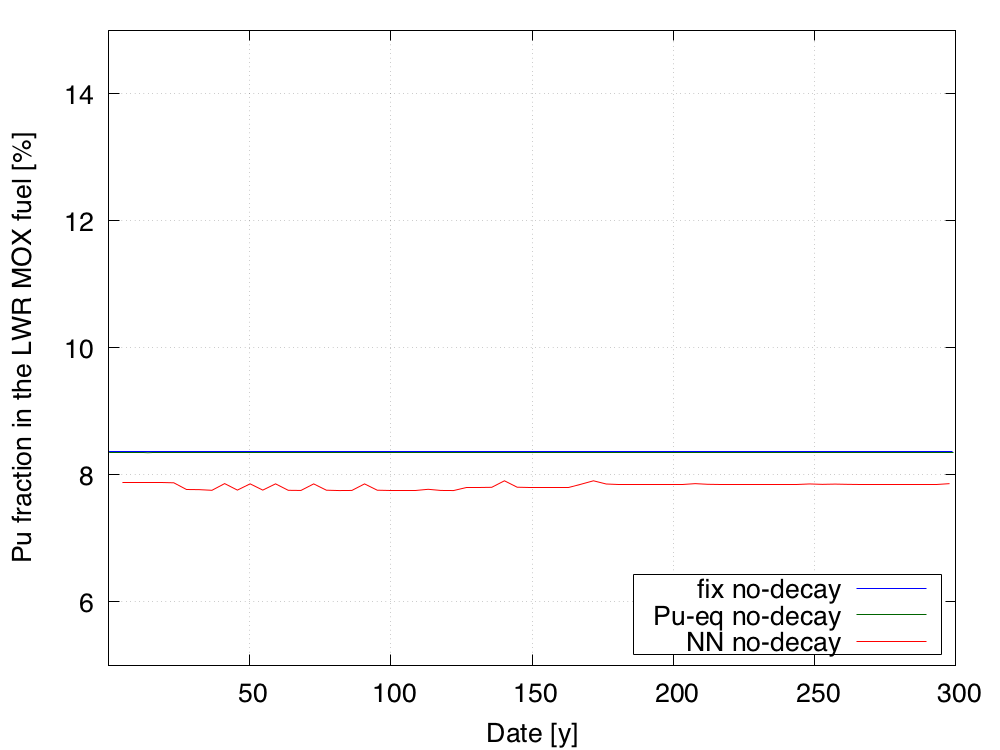
\includegraphics[width=0.48\textwidth]{nodecay_pu_contribution.png}
  \caption{Evolution of the fraction of plutonium in the fresh PWR-MOX fuel
  using the 3 predicted models, without considering decay.}
  \label{fig:nod}
\end{figure}


Activating decay, see Fig. \ref{fig:d}, results for the ``fix mixing ratio''
calculation in a small decrease of the fraction of plutonium in the fuel,
corresponding to the decay of $^{241}$Pu into $^{241}$Am. For the
``Pu-equivalent'' modeling we can observe a slight increase of the fraction of
plutonium, which is required to compensate for the negative reactivity effect
coming with the $^{241}$Am. For the calculation using ``Neural network'' fuel
fabrication modeling the effect is very quickly increasing to $13\%$ and then
slowing stabilising while the plutonium inventory reach an equilibrium\ldots

\begin{figure}[ht] % replace 't' with 'b' to force it to be on the bottom
  \centering
  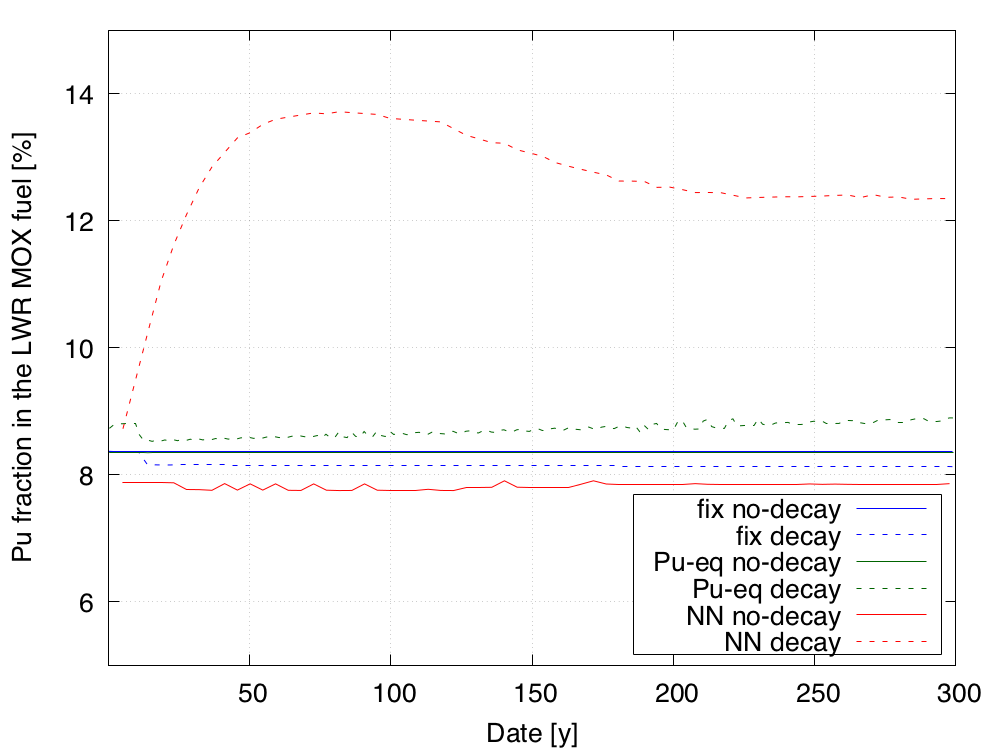
\includegraphics[width=0.48\textwidth]{decay_pu_contribution.png}
  \caption{Evolution of the fraction of plutonium in the fresh PWR-MOX fuel
  using the 3 prediction models, with and without decay enable.}
  \label{fig:d}
\end{figure}

As the calculation using ``Neural Network'' fabrication modeling, requires more
plutonium than the cycle can produce, the initial inventory has been set to an
higher values, increasing the plutonium decay effect. Nevertheless this shows
the strong impact of the presence of $^{241}$Am with the plutonium used for the
PWR-MOX fuel fabrication.

A last calculation, on decay have been performed using the ``Pu-equivalent''
fabrication model, increasing by a factor 2, 5 and 10 the amount of plutonium in
the startup inventory, trying to mimic different degree of a plutonium pill-up.
This calculation shoes an change from 10 to 30\% in the mixing ratio required to
build the proper PWR-MOX fuel. Those kind of plutonium pilling up can
unexpectedly occurs in a real fuel cycle and might need to be considered in a
complete fuel cycle transition study.

The decay process tends to change to composition of the plutonium vector, and
then of the plutonium enrichment require to build a proper PWR-MOX fuel. Those
composition change in the MOX fuel will impact the individual cross section:
specially in thermal reactor where the macroscopic cross section are very
dependent on the shape of the thermal part of the neutron spectrum, which is
strongly driven by the fuel isotopic composition.


%%%%%%%%%%%%%%%%%%%%%%%%%%%%%%%%%%%%%%%%%%%%%%%%%%%%%%%%%%%%%%%%%%%%%%%%%%%%%%%%
\section{Depletion vs Recipe}

This part is dedicated to the evaluation of the impact of the depletion
calculation in a fuel cycle macroscopic level.

\begin{figure}[ht] % replace 't' with 'b' to force it to be on the bottom
  \centering
  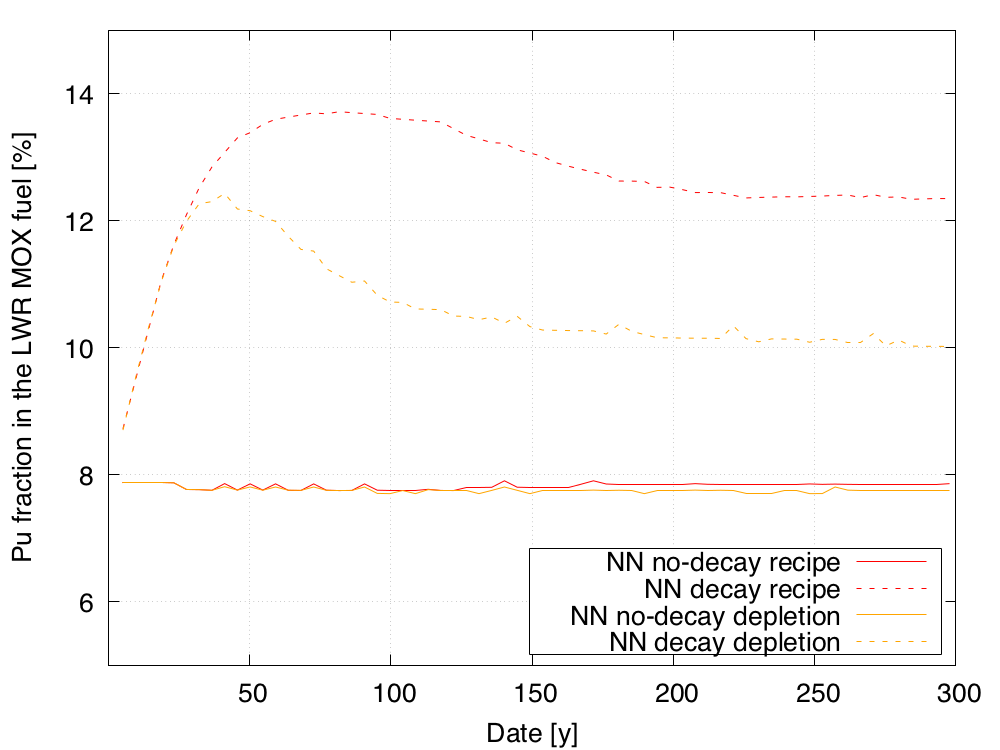
\includegraphics[width=0.48\textwidth]{irradiation_pu_contribution.png}
  \caption{Evolution of the fraction of plutonium in the fresh PWR-MOX fuel
  using the ``Neural Network'' prediction models, with decay enable using recipe
based spent fuel composition and recalculated spent fuel composition.}
  \label{fig:depletion}
\end{figure}

Two additional calculations have been performed. Those calculations use the
neural network for the fuel fabrication modeling as well as for the
recalculation of the MOX fuel depletion calculation: for each MOX fuel loaded in
the reactor, a dedicated depletion calculation also to update the output recipe
used for the spent MOX fuel.


As shown on Fig. \ref{fig:depletion}, the equilibrium values for recipe based
calculation and the depletion calculation are not the same. Moreover,
recalculating the fuel spent fuel composition for each loaded fuel allows the
cycle to reach faster its equilibrium. 

This is led by the slight change in the composition in the available plutonium
(see Fig. \ref{fig:depletioncompo}): in the case of the depletion calculation
the available plutonium contain $68\%$ of $^{239}$Pu versus $64\%$ in the recipe
based case, and also significantly less $^{241}$Pu leading to less $^{242}$Pu in
the cycle. The amount of the other nuclide are very close.

\begin{figure}[ht] % replace 't' with 'b' to force it to be on the bottom
  \centering
  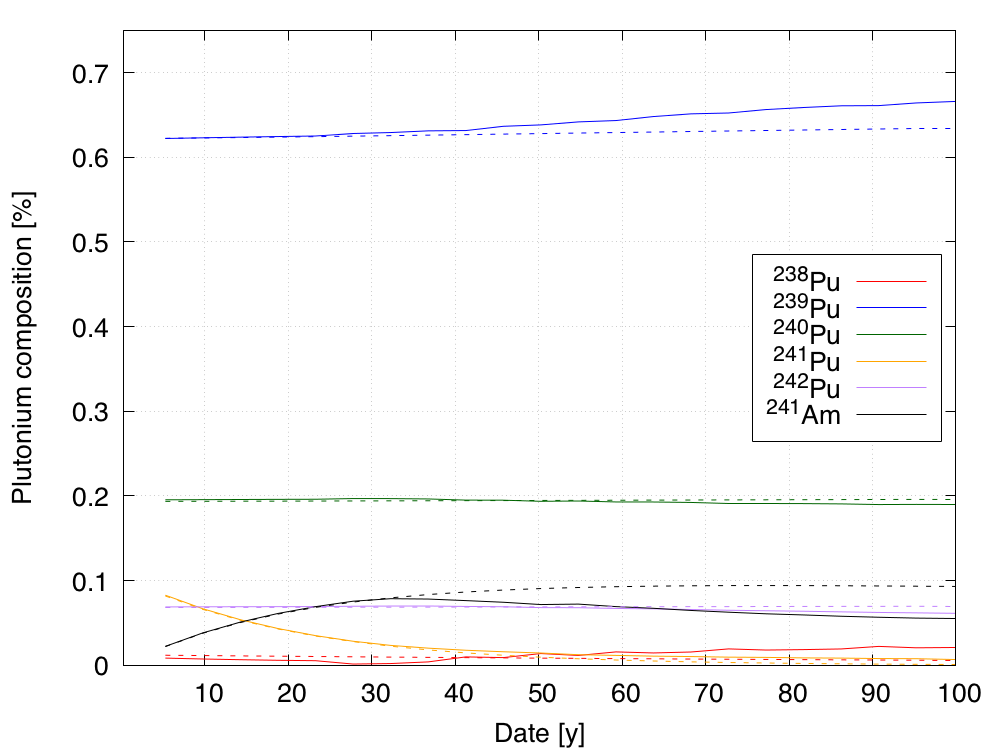
\includegraphics[width=0.48\textwidth]{MOX_pu_composition.png}
  \caption{Evolution of the composition of the plutonium in the fresh PWR-MOX fuel
  using the ``Neural Network'' prediction models, with decay enable using recipe
based spent fuel composition and recalculated spent fuel composition.}
  \label{fig:depletioncompo}
\end{figure}

Those slight change in the output composition, lead to an overall decrease of
the amount of $^{241}$Am in the fresh PWR-MOX fuel and an increase of the
$^{239}$Pu, allowing to build fuel with a lower plutonium enrichment.


%%%%%%%%%%%%%%%%%%%%%%%%%%%%%%%%%%%%%%%%%%%%%%%%%%%%%%%%%%%%%%%%%%%%%%%%%%%%%%%%
\section{Conclusions}

This study have shown the potential impact of the decay process on the MOX-PWR fuel
fabrication process, increasing the required amount from $1\%$ to $4\%$
depending on the fuel fabrication modelization. The recalculation of the 
depletion of each loaded fuel has for consequences the change of the equilibrium
state of the calculation: the reduction of fraction of $^{241}$Am and the increase of the
fraction $^{239}$Pu in the available plutonium allows to reduce the amount of
plutonium at an alternate level (between the no-decay calculation and the recipe
based calculation). 

This work has shown the strong influence of the isotopic composition on a LWR
cycle involving plutonium recycling. Similar analysis will be conducted in the
near future on the FBR part of the EG29 fuel cycle, which should be less
impacted by those isotopic changes, as fast spectrum reactor are less sensitive
to those change.

Moreover this study has shown the potential of a agent based fuel cycle tool
such as Cyclus. Not only Cyclus follows every isotopes in the cycle,
but its modularity allows also to add modules based on other tool technology such
as the Neural networks model developed for the French fuel cycle tool, CLASS.
Those quality made of Cyclus a great platform to do such comparative study
allowing to only change a specific aspect of the fuel cycle description while
keeping every thing else identical.






%%%%%%%%%%%%%%%%%%%%%%%%%%%%%%%%%%%%%%%%%%%%%%%%%%%%%%%%%%%%%%%%%%%%%%%%%%%%%%%%
%\appendix
%\section{Appendix}
%
%Numbering in the appendix is different:
%\begin{equation} \label{eq:appendix}
%  2 + 2 = 5\,.
%\end{equation}
%and another equation:
%\begin{equation} \label{eq:appendix2}
%  a + b = c\,.
%\end{equation}

%%%%%%%%%%%%%%%%%%%%%%%%%%%%%%%%%%%%%%%%%%%%%%%%%%%%%%%%%%%%%%%%%%%%%%%%%%%%%%%%
\section{Acknowledgments}
Shall we acknowledge anyone ? DOE ? FCO ?


%%%%%%%%%%%%%%%%%%%%%%%%%%%%%%%%%%%%%%%%%%%%%%%%%%%%%%%%%%%%%%%%%%%%%%%%%%%%%%%%
\bibliographystyle{ans}
\bibliography{bibliography}
\end{document}

